\documentclass{article}

\usepackage[final]{neurips_2019}

\usepackage[utf8]{inputenc}
\usepackage[T1]{fontenc}
\usepackage{hyperref}
\usepackage{url}
\usepackage{booktabs}
\usepackage{amsfonts}
\usepackage{nicefrac}
\usepackage{microtype}
\usepackage{graphicx}
\usepackage{xcolor}
\usepackage{lipsum}
\usepackage{tikz}
\usepackage{pgfplots}

\newcommand{\note}[1]{\textcolor{blue}{{#1}}}

\title{
  Inside-Out Code Auto-Completion \\
  \vspace{1em}
  \small{\normalfont Stanford CS224N Custom Project}  % Select one and delete the other
  \\
  \small{\normalfont Mentor: Mina Lee}  % Select one and
  \\
  \small{\normalfont Grading option: 3 (graded)}  % Select one and

}

\author{
  Gabriel Poesia \\
  Department of Computer Science \\
  Stanford University \\
  \texttt{poesia@stanford.edu} \\
  \And
  Lauren Gillespie \\
  Department of Computer Science \\
  Stanford University \\
  \texttt{gillespl@stanford.edu} \\
  \And
  Scott Viteri \\
  Department of Computer Science \\
  Stanford University \\
  \texttt{sviteri@stanford.edu}

}

\begin{document}

\maketitle

\begin{abstract}
  Auto-complete has become a ubiquitous feature in modern-day typing systems. Traditional systems typically try to predict the next characters or words the user is about to type. In contrast, keyword-based auto-completion systems expect the user to type keywords,
   then fill in the least informative parts of the sentence, and have been successful
  for a variety of natural language tasks. In this project, we implement a keyword-based auto-complete technique for programming languages,
  as auto-complete systems in modern IDEs are still mostly left-to-right. We use three programming
  languages with different verbosity levels: Python, Haskell and Java. We evaluate different encoding schemes paired
  with a neural decoder with various trade-offs in translation accuracy and compression, and evaluate their accuracy and robustness.

%   , and show that the obtained
%   models can find a reasonable balance between accuracy
%   and the number of characters that users do not
%   need to type when such a system is in place.
\end{abstract}

% {\color{red} This template does not contain the full instruction set for this assignment; please refer back to the milestone instructions PDF.}

\section{Introduction}
Auto-complete has become a ubiquitous feature in almost all modern-day typing systems. However, almost all of these auto-complete systems utilize left-to-right (LTR) predictive auto-completion. Yet the most important information in a sentence or phrase isn't guaranteed to be clustered at the beginning. A more efficient system instead would enable users to convey the most important information of the sentence or phrase in the form of keywords, so instead of predicting the rest of the sentence from left-to-right, the system predicts the the full sentence from its keywords, in an \textit{inside-out} fashion.

For example, in the LTR setting, if a user wants to communicate the sentence ``I want to see Lion King at 10 o'clock pm'' she will to first type ``I want to see''. Even then, it will be difficult for the system to infer the rest of the sentence, since the first few words have such low information density. In the keyword-based setting the user might only have to type ``Lion King 10 pm''.

Similar bottlenecks occur when programming. For example, to when typing \texttt{for i in range(10):} Pythia\footnote{a left-to-right auto-complete system} only auto-completes \texttt{for i in r} to \texttt{for i in range}, and \texttt{(10)} is manually typed. However, typing \texttt{for i in 10} would convey the same information to a human user in fewer characters. A keyword-based system might be able to auto-complete this shorthand.

In this paper, we describe and analyze a character-level auto-complete system for
lines of source code. We experiment with several
choices that place an auto-completion scheme in
the compactness-accuracy spectrum. In Section 2,
we survey related work. Section 3 formalizes the
auto-completion problem and explains our solution.
Section 4 describes our experimental setup.
Section 5 discusses the results and examples from
the various proposed auto-completion schemes.
Finally, Section 6 summarizes our results.

% from michael's book: Sloppy programming also offers benefits to expert programmers as an extension to autocomplete, by decreasing the cognitive load of coding in several ways. First, sloppy queries are often shorter than code, and easier to type. Second, the user does not need to recall all the lexical components (e.g., variable names and methods) involved in an expression, because the computer may be able to infer some of them. Third, the user does not need to type the syntax for calling methods. In fact, the user does not even need to know the syntax, which may be useful for users who switch between languages often.

%  To do so, we train a seq-to-seq decoder that is jointly trained with a context sensitive encoder to convert keyword-based compressions of a line of code to its full representation. <TODO: add some more here about our system> Previous keyword-based code auto-completion systems are language-specific and
% context sensitive encoder is better for training the end-to-end model because it creates a more human-like compressed and also denser representation than our baselines
% the introduction gives more space for motivation, detail, references to existing work, and to capture the reader's interest.

\section{Related Work}
Previous work implemented a neural-based auto-complete system for natural language tasks\cite{lee2019learning}. This system implements a context-sensitive neural encoding scheme which compresses target sequences. While Lee et. al. implements inside-out auto-completion for natural language tasks, our system specifically focuses on programming language implementation of inside-out auto-completion.

Little et. al. also proposed a keyword-based Java auto-complete system\cite{Little2009}. However, their system only generates method calls, variable references, and constructor calls, while ours generates arbitrary lines of code. Their implementation operates on a word level, while ours is character-based. Also, their system is not robust to abbreviations of keywords themselves; the system cannot match keywords that are not character-for-character present in the table of keywords translations. Finally, their system is language-specific while our proposed method is language-agnostic.

Reiss 2009 implements a keyword-based function generator for Java code \cite{Reiss}. In this system keywords are used as search keys into a database of existing programs, and matched programs undergo a series of program transformations. These program transformation must be written separately for each language. The main purpose of this program is to search for pre-existing programs, rather than generate wholly new ones.

%Pandita et. al. %
%<talk about search -related keyword autocomplete?>

%<Beyond autocomplete: Automatic function definition>

%Semantics-based code search>
%<improvement and Implementation of Keyword Programming> ummm cant get this cause apparently you ahv eto be polish??


\section{Approach}

% Problem statement: given a string S, abbreviate it into a subsequence T of S, predict original string S from T. Want T to be small, yet prediction to be correct.
We now describe our approach in building a code auto-complete system.
We define an \emph{auto-completion scheme}
$A$ to be a pair of functions $A = (E, D)$, both mapping strings to strings. Suppose the user wants to
type a certain string $s$. By applying the \emph{encoder} of $A$, we get $s' = E(s)$, a string that
the user can type instead of the potentially longer $s$, and use the decoder function $D(s')$ to get
back the original string $s$.

Two features would be desired of a scheme $A$.
First, we would like the encoded strings to be small, as the overall goal is to save the user typing
effort. More precisely, we want $\mathbb{E}_{s \in C} |E(s)|$ to be as small as possible, where
the expectation is taken over the probability distribution of lines of code in a certain
programming language.
Furthermore, we want the decoder to be able to precisely determine the original line of code
after it has been encoded, i.e. we want $\mathbb{E}_{s \in C} \left(\mathbb{P}(s = D(E(s))) \right)$
to be as close to $1$ as possible. These two goals are clearly conflicting: the most precise encoding
scheme would be the identity scheme, which is not compact, while any scheme that shortens the input
will introduce uncertainty in the decoding. We therefore study several auto-completion schemes that
fall into different points of this trade-off.

Finally, we also want an auto-complete scheme to be
intuitive to users. A compact and precise scheme could
be built by assigning common lines of code to short sequences of characters that rarely occur in real code (or even do not belong to the programming language at hand). To keep the encoded strings related to the user's intent,
as in \cite{lee2019learning} we restrict ourselves to
encoding schemes that output a \emph{sub-sequence} of the
input characters. In other words, the encoder can only drop, but not
add, characters to the input.

\subsection{Encoder}

The \emph{encoder} side of an auto-complete scheme aims
at dropping the least informative characters in such a
way that the decoder is still able to recover the input.
We consider two kinds of encoders: \emph{ad hoc} encoders,
which are plain algorithms that a neural decoder is trained
to invert, and a \emph{neural context-sensitive}
encoder that is trained end-to-end alongside the decoder.
We designed the following \emph{ad hoc} encoders:

\begin{description}
    \item[Rules. ]{Many programming languages have common commands that are long to type. For example, to write a line to the standard output in Java, one would use the \texttt{System.out.println()} method (or a similar alternative). From a list of such common commands and keywords, several modern Integrated Development Environments (IDEs) have
    a table of intuitive abbreviations that expand to
    the long commands. Some Java IDEs, for instance,
    expand \texttt{sout} to \texttt{System.out.println}, which users can easily memorize.
    Our \emph{Rules} encoder applies a manually-crafted
    table of abbreviations to the input lines of code.
    Examples of abbreviations we have for Python are
    \texttt{T} $\rightarrow$ \texttt{True} and
    \texttt{rev} $\rightarrow$ \texttt{reverse}.
    }

    \item[Uniform. ]{
    While \emph{Rules} is very intuitive, it is also
    very rigid, as all abbreviations are defined
    \emph{a priori}. On the other extreme, we can
    think of simply dropping characters at random.
    This is the \emph{Uniform} encoder, which is
    parameterized by the probability $p$ of dropping
    each character, independently. Therefore,
    \emph{Uniform} can abbreviate any string $s$
    into a string that has expected length $p \times |s|$.
    }

    \item[Frequency. ]{
        The flexibility of \emph{Uniform} also has a
        cost: while it's easy to identify common
        sequences of characters like \emph{System.out.println} even when any
        $30\%$ of the characters are removed, rarer
        sequences are hardly identifiable, as there
        are few examples of them. The same happens
        for short sequences (like operators) that
        might be entirely erased during encoding.
        As a balance between the focus of \emph{Rules}
        on frequently-used keywords and the breadth
        of \emph{Uniform}, the \emph{Frequency}
        encoder first ranks character $n$-grams by
        their frequency in the training set, and then
        replaces $n$-grams by a concatenation of
        their first and last characters until the length
        of the input is reduced to a desired fraction $p$. For example, if $p = 0.8$, the length
        of the input is reduced by $20\%$.
        After some experimentation, we decided
        to use $n = 5$ as our $n$-gram size.
        One example of a rule that the
        \emph{Frequency} encoder uses is
        \texttt{print} $\rightarrow$ \textt{pt}.
    }
    \item[Noisy Frequency. ]{
        While a system trained with
        \emph{Frequency} achieves a good
        compression rate and accuracy, in practice we
        observed this encoder is not robust to
        the user using different abbreviations
        than the first and last characters of the
        $n$-gram (we show this analysis in
        Section~\ref{sec:experiments}). This is important for use in the
        real world, as we also want users not to have
        to need much adaptation to use the system.
        With this motivation, we devised the
        \emph{Noisy Frequency} encoder, which is
        also parameterized by the desired fraction $p$
        of characters to be kept. The goal is to train
        \emph{Frequency} to be also robust to noise.
        Starting from the
        input, in each step this encoder either removes
        one character at random or applies the
        same rule as \emph{Frequency} that abbreviates
        one $n$-gram. Both options are equally likely
        and subsequent decisions are independent.
    }
\end{description}

% Context-Senstive Encoder
Besides these \emph{ad hoc} encoders, we also
implemented a \emph{neural context-sensitive}
encoder that is trained end-to-end with the decoder.
We use the same model as Lee et al. \cite{lee2019learning}, where an LSTM model
outputs a probability of dropping each character
in the input. We then sample from that probability
distribution to get the encoded string, which is
then fed into the decoder that tries to reconstruct
the original output. Unfortunately, despite our
best efforts, we did not manage to get useful results
out of this model. While we used their same
constrained objective function, we still got the results that are reported for the less stable linear objective, where the encoder degenerates during
training to either
keep all characters (minimizing the decoder loss) or drop all characters (minimizing
the average length of the encoded strings).
We suspect that, since our system is character-level,
which makes input sequences significantly larger than the ones this encoder architecture was originally
designed for, the model might take more time to
leave trivial local minima than what we had available. Therefore, all results and analyses we show only
consider \emph{ad hoc} encoders.

\subsection{Decoder}

We pair all described encoders with
a neural decoder implemented as a standard
sequence-to-sequence architecture with
multiplicative attention, where
the input (the abbreviated string)
is first encoded by a bidirectional LSTM,
and then decoded into the expanded string
by a uni-directional LSTM. We jointly train character embeddings with our models, which
was observed to be better than using one-hot
encodings.

\subsubsection{Attention-based copy mechanism}

As in \cite{lee2019learning}, we also integrated a \emph{copy mechanism} in our
model, as described in \cite{copy_mech}.
We observed that the model begins training
with a smaller loss than without copy,
but the final accuracy is decreased
by 10\% on average in all settings.
After analyzing
running examples, we observed that the
attention distribution is not precise
enough in the case of a character-based
code model to inform the characters to be
written to the output.

We notice that there are significant differences
between our use case and the scenario
that attention-based copy was designed
for. First, the sequences
of characters we deal with are on average
much longer than the number of tokens
in a typical sentence in natural language.
More precisely, our average line of Python
code had $36.5$ characters, whereas the
auto-complete system in \cite{lee2019learning} was only tested
in sequences of at most $16$ tokens.
Also, the alphabet size in our case
is $128$, from ASCII encoding: much smaller than the tens of thousands of words that are
typically used in the vocabulary of
natural language systems. These differences
likely make attention-based copy mechanisms
inappropriate to our case, and therefore
we did not use it in our final model.

\subsubsection{\emph{Hard-copy} mechanism}

Motivated by the fact that the output
of the decoder is a super-sequence of
its input, we designed a custom
\emph{hard-copy}
mechanism that is not attention-based.
If the original input had $n$ characters
and the encoded input has $n' < n$ characters, we know at training time that
the decoder has to copy all $n'$ characters
from its input at some point, and also insert $n' - n$ characters in between.
Furthermore, we know that the copied
characters will come in order, and because
we know which characters were removed,
we can also compute the expected sequences
of actions of the decoder, being either
to insert a character or copy the next
character from the input. For example,
if the string \texttt{print} was shortened
to \texttt{pt}, we expect the decoder to
first copy \texttt{p}, then do three insertions of \texttt{r}, \texttt{i}
and \texttt{n} and finally copy \texttt{t}.

We experimented with augmenting the decoder
output with a special character that triggers
a copy of the next character from the input
that has not yet been copied.
In this way, the copy is \emph{non-parametric},
i.e. the model doesn't need to specify which
character to copy.
We observed that,
at first, if the minority of the
characters are dropped by the encoder,
most of the expected output characters are the
special ``copy'' token, and the decoder quickly
learns to always copy at every step.
Under this framework, the model can
achieve zero loss on all characters that
have not been dropped if it outputs
a probability of $1$ to the copy character
at all time steps. Thus, it gets stuck
at this local optimum of only copying the compressed representation, which clearly
fails in all test examples where at least
one character was removed. If we drop
more than the majority of the characters,
the model does not learn to output ``copy''
at all time steps, but also doesn't learn
useful associations as the compressed representation simply
contains too little information to predict
the original line. We therefore
ended up not using this \emph{hard-copy}
mechanism in our decoder.

\section{Experiments}
\label{sec:experiments}

We evaluated all \emph{ad hoc} encoders described
in Section~3, paired with the neural decoder. Our investigation is guided
by three research questions:

\begin{description}
    \item[RQ1: ] How do the different auto-complete schemes compare in accuracy and robustness?
    \item[RQ2: ] What is the impact of
    the compression rate of an
    auto-complete scheme in its
    accuracy?
    \item[RQ3: ] How do different
    programming languages impact the
    accuracy of auto-complete systems?
\end{description}

\subsection{Data}

We built a dataset comprised of code extracted from public GitHub repositories written in Python, Haskell, and Java.
We ignored comments,
indentation and lines that
are either fewer than 10 or greater than 80 characters long. In total,
for each programming language,
we used 600k unique lines
of code for training,
80k for validation and
hyper-parameter tuning,
and 80k for testing.

\subsection{Experimental Details}

All experiments were executed
on a Intel(R) Xeon(R) E5-2690
machine running
Ubuntu Server 16.04,
with 56GB of RAM,
and a single NVIDIA Tesla M60 GPU
with 8GB of memory.

For the neural decoder, we used
a 512-dimensional single-layer LSTM model. We jointly trained
50-dimensional character
embeddings with each
encoder-decoder pair.
Each model was trained for
4h using the Adam
optimizer, with a learning
rate of 0.0001,
$\beta_1 = 0.9$ and $\beta_2 = 0.999$.

We trained all 4 \emph{ad hoc} encoders described
in Section 3. For \emph{Uniform}, \emph{Frequency} and \emph{NoisyFrequency}, we set their parameter $p$ to $0.8$ unless noted otherwise,
which means \emph{Uniform} drops each character
independently with probability $0.2$, and \emph{Frequency}
and \emph{NoisyFrequency} remove characters until the input
is reduced by at least $20\%$. Finally,
\emph{Frequency} and \emph{NoisyFrequency} are always set to operate on character $5$-grams.

\subsection{Accuracy and Robustness of Auto-Complete Schemes}

\begin{table}
\centering
\begin{tabular}{|l|l|l|l|l|}
\hline
                    & Rules Dec.     & Uniform Dec.  & Frequency Dec. & NoisyFrequency Dec. \\ \hline
Rules Enc.          & 0.943 / 0.980  & 0.643 / 0.805 & 0.210 / 0.385  & 0.182 / 0.450       \\ \hline
Uniform Enc.        & 0.008 / 0.015  & 0.181 / 0.340 & 0.002 / 0.010  & 0.070 / 0.250       \\ \hline
Frequency Enc.      & 0.000 / 0.005  & 0.077 / 0.270 & 0.592 / 0.765  & 0.037 / 0.115       \\ \hline
NoisyFrequency Enc. & 0.000 / 0.000  & 0.020 / 0.060 & 0.000 / 0.000  & 0.248 / 0.410       \\ \hline
\end{tabular}
\bigskip
\caption{Top-1 Accuracies / Top-5 Accuracies for Encoder/Decoder Pairs.}
\label{tab:top1accnoisy}
\end{table}

To compare the different
proposed auto-complete schemes,
we first trained neural decoders for each all 4
encoders: \emph{Rules, Uniform, Frequency} and \emph{NoisyFrequency}.
Then, we split each scheme
into an encoder-decoder pair,
and evaluate all decoders
when running on the output
of all encoders. Ideally,
an auto-complete scheme should
be accurate when its encoder
and decoder are paired, but
we'd also like the decoder
to be robust and be able to
correctly reconstruct input
abbreviated by different
encoders, as we cannot expect
all users to use the
same abbreviations.

Table~\ref{tab:top1accnoisy}
shows the accuracies of both
top-1 and top-5 predictions
for all encoder/decoder pairs.
We note that \emph{Rules} is
very accurate on itself, having
a \emph{98\%} top-5 accuracy. However,
a decoder only trained along
the \emph{Rules} encoder
is not robust: its top-5 accuracy
is at most $2\%$ for other
encoders. \emph{Frequency} decoder
has a high accuracy when the
input comes from the corresponding
encoder ($76.5$\% top-5 accuracy),
but it is not robust: its top-1
accuracy drops to zero on both
\emph{Uniform} and \emph{NoisyFrequency}. This indicates
that it cannot perform
expansions that are not in
the computed table of
frequent $n$-grams.

As expected, \emph{NoisyFrequency}
is slightly more robust,
having its worst top-5 accuracy
of $11.5$\% on the \emph{Frequency} encoder. Surprisingly, its accuracy
increases when paired with the
\emph{Uniform} encoder, going up to
$25$\%, suggesting that the
noise makes the model not specialize to frequent $n$-grams necessarily.
Finally, \emph{Uniform} decoder has the best performance on the \emph{Rules} encoder besides its across all decoders other than \emph{Rules} itself.
This suggests that \emph{Uniform} successfully learns to pick up common-sense patterns,
even though it is trained on purely random abbreviations.

These results indicate a positive correlation between the regularity of an encoder
and the accuracy of its decoder, but this accuracy trades-off with robustness.
\emph{Rules} is the most predictable encoder, and therefore leads to the most
accurate auto-complete scheme; however, it is the least robust. On the other extreme,
\emph{Uniform} has the worst result on itself, but was shown to be more robust than
other schemes, and is able to decode \emph{Rules} fairly accurately even without
specialized training. These observations answer our first research question.

\subsection{Impact of compactness on accuracy}

We now aim at understanding the impact of the compactness
of an auto-complete scheme on its accuracy.
To that end, we trained \emph{Uniform} decoders
with four different probabilities of keeping each character:
$0.6$, $0.7$, $0.8$ and $0.9$.
Figure~\ref{fig:unif} shows the top-1 accuracies of each
of the obtained decoders when expanding input that was
compressed to each of these sizes.

\begin{figure}
    \centering
    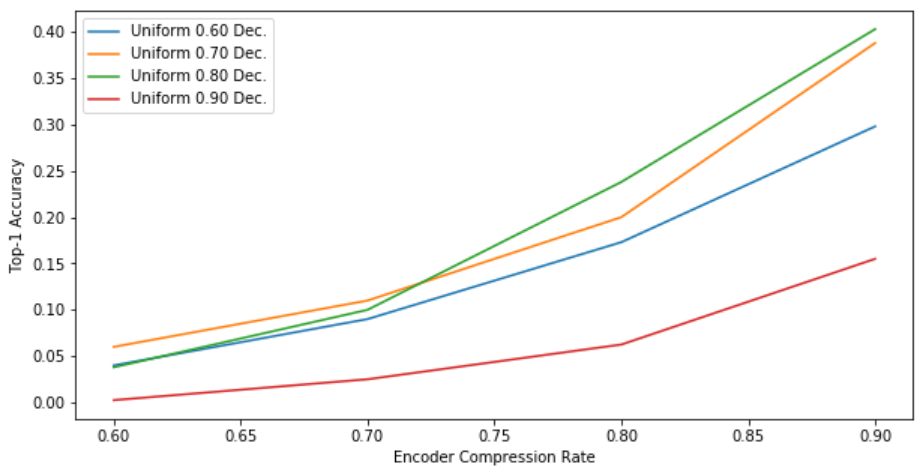
\includegraphics[width=0.9\textwidth]{template/plot_unif.png}
    \caption{Top-1 accuracy of \emph{Uniform} decoders trained
    with different compression rates.}
    \label{fig:unif}
\end{figure}

First, we note that the learned \emph{Uniform} decoders
do not overfit the relationship between the length of the
input and the length of the output, which has a fixed
average during training. For example, for \emph{Uniform 0.8}
decoder, if the input has $8$ characters, it could
potentially expect the output to have $10$ characters
based on its training procedure. However, in practice,
this does not happen. As one would desire, the performance
of all decoders increase monotonically when we drop less
characters. The worst performance of all decoders happen
when the input has only $60\%$ of the original characters.
When $90\%$ of the input is kept, the decoders
perform at their best.

Also, we notice an interesting relationship between robustness
of the learned scheme and the amount of noise present in
the input. All decoders have a higher accuracy than
\emph{Uniform 0.9} when $90\%$ of the characters are kept,
even if \emph{Uniform 0.9} decoder was specialized for this
case. This suggests that seeing more noise in the input
helps other decoders in easier cases as well. On the
other extreme, \emph{Uniform 0.6} performs worse
than \emph{Uniform 0.7} and \emph{Uniform 0.8} when
\emph{90\%} of the characters are kept on average.
As much as noise helps in robustness, too much noise
can also hinder the decoder from learning useful representations. Most likely, \emph{Uniform 0.7} and $0.8$
are closer to the sweet spot in the amount of noise during
training, since their performance was mostly equivalent
on all noise scenarios and superior to the other two decoders.
This result provides insight to answer our second
research question.

\subsection{Impact of different programming languages on auto-complete schemes}

Finally, we evaluate how different programming
languages impact the performance of auto-complete
schemes. First, we notice that the average line length
of a programming language determines how many characters
are dropped on average by \emph{Uniform}, which alone
makes it easier or harder to recover all dropped
characters accurately.
Among the 3 languages we analyze, Python
has the smallest average line length, at $35.4$ characters.
Haskell is a close second, with $35.9$, while Java
has the longest average lines, with $39.3$ characters.
To let this difference aside, in this experiment we
instead drop a constant number of $5$ characters of each
line, instead of a variable fraction of the input.

Table~\ref{tab:top1acclangs} shows top-1 accuracy results
for all 3 programming languages, and also for different
line lengths. Of these 3 languages, Haskell is commonly
known as the most concise, and Java as the most verbose.
Our results match this common perception: even though
line lengths for Haskell and Python are very similar
on average, it is significantly harder to auto-complete
Haskell code. When analyzing individual lines, we see
a larger prevalence of one-character names in that language,
for example. When such a character is dropped, it is
not reasonable to expect it to be recovered by the decoder.
This makes longer lines harder in Haskell than shorter
lines, because there are more opportunities for making
this kind of mistake. The same phenomenon is observed
in Python. In Java, however, longer lines are easier
for the decoder than shorter lines. We noticed that
the longest Java lines usually contain common long
class names, such as \texttt{ConcurrentHashMap}
or \texttt{BufferedOutputStream}, which tend to appear
twice in the same line in variable declarations.
Therefore, longer lines in Java tend to have more
redundancy than longer lines in Python or Haskell,
which are usually very dense. These results let us
conclude that it is significantly easier to build accurate auto-complete systems for more verbose programming languages.
This answers our third research question.

\begin{table}
\centering
\begin{tabular}{|l|l|l|l|l|}
\hline
            & Python & Java  & Haskell \\ \hline
All lines   & 0.201  & 0.353 & 0.154   \\ \hline
Short lines & 0.182  & 0.239 & 0.124   \\ \hline
Long lines  & 0.174  & 0.373 & 0.120   \\ \hline
\end{tabular}
\bigskip
\caption{Top-1 Accuracies for \emph{Uniform} trained with constantly dropping 5 characters for Python, Java, and Haskell. Long lines contain more than 65 characters and short lines contain less than 25 characters.}
\label{tab:top1acclangs}
\end{table}

\section{Analysis}
Suppose the user wants to type \texttt{for i in range(10):}. The rules-based decoder correctly translates \texttt{for i in rng(10):} to \texttt{for i in range(10):}, but incorrectly translates \texttt{for i in rg(10):} to \texttt{for i in rg(10):}.
Rules-based works for the abbreviation 'rng', because it was explicitly in the translation list. But if the abbreviation is not on the list, the decoder struggles: the rules-based decoder will only work on a small range on abbreviations. We want our model to be flexible with respect to the various encodings that a programmer might use.

One way to ensure flexibility is to separately decide whether to drop each character with some fixed probability -- the uniform encoder at 0.8 dropout probability correctly expands both \texttt{for i in rng(10):} and \texttt{for i in rg(10):}.

But we are still missing something in our model of how humans would choose to omit characters when using our auto-completion framework. Certain characters are more likely to be dropped in accordance with how redundant they are semantically -- we approximate this using our \emph{Frequency} encoder.

Consider the Python line \texttt{parser.add\_option("-v", "--version", help="use a specific zc.buildout version")}, and the encoding \texttt{per.\_opn("-v", "--vern", help="use a specific zc.bdout vern")}. \emph{Uniform} incorrectly decodes to \texttt{per.\_open("-v", "--version", help="user a specific zc.bidout version")}, while \emph{Frequency} decoder expands it correctly. The common 5-grams that were identified in the original string were 'parse', '.add\_', 'ption', 'rsion', 'build', and 'rsion' again. The uniform case does not reconstruct 'zc.buildout' from 'zc.bdout' because it treats the deletion of 'u','i', and 'l' as independent events, and therefore underestimates the true probability of dropping all three.

The frequency-based decoder sees 10, and guesses that it really comes from the sequence 10000. Even worse, in the beam search the number is further expanded because it thinks that 00 comes from 00000.

This could be due to the decoder learning that it needs to expand the input string, and will prefer longer explanations as a result. The frequency-based decoder's strength is building translations using fairly non-local information; however, the price is that it tends to violate Occam's Razor.

We would like to evaluate these models, but accuracies of different models each using their own encoding schemes are somewhat incomparable. For example, a rule-based encoding is much easier to expand than a uniform encoding. A uniform decoder would have to be very powerful to score as well on uniform encodings as rule based decoder performs on its rule based encodings. We also need to understand which of the encoding schemes is closest to what programmers would actually type when using these auto-completion facilities.

As Table~\ref{tab:top1accnoisy} shows, \emph{Rules} decodes its own encodings nearly perfectly, but cannot decode uniform or frequency -- it is overfitting to its own very simple encodings. We can see the simplicity of the rule-based encodings in the high uniform and frequency based decoding scores.

The uniform decoder performs meagerly on its own encodings, but performs well on rule-based encodings. The uniform decoder always performs at least tolerably on \emph{Frequency},
with a $27\%$ top-5 accuracy. The uniform decoder can be viewed as underfitting its own encoder, partially because the uniform encoder is especially difficult to reliably decode.

Contrast this with the frequency decoder. It performs well on itself and reasonably on rule-based, but it completely fails on uniform encodings. In other words, it is overfitting its own encoder. The frequency decoder is inflexible -- a small perturbation causes it to leave the regime where it can give confident predictions. This is because the frequency encoder is forced to only consider fixed deletions of n-grams in a fixed order, given by relative n-gram frequencies in the dataset\footnote{With the caveat in choosing which of multiple equivalently prevalent n-grams to choose}.

We can find a middle ground between the under and over fitting of uniform and frequency based encoders respectively by introducing noise into the frequency encoding, as we did in our \emph{NoisyFrequency} encoder.

To really get a feel for the efficacies of these learned decoders we will need to see examples.
Consider translations of \texttt{for i in rng(10):} in
Table~\ref{tab:translations}.

\begin{table}[h!]
\centering
\begin{tabular}{|l|l|l|l|l|}
\hline
Rules  & 'for i in range(10):' & 'for i in range(10):ul::' \\ \hline
Uniform  & 'for i in range(10):' & 'for i in range(100):'    \\ \hline
Frequency  & 'for i in rading(10):' & 'for i in rng(10000):'   \\ \hline
NoisyFrequency & 'for i in range(10):' & 'for i in range(100):'    \\ \hline
\end{tabular}
\bigskip
\caption{Top-2 Translations for the input \texttt{for i in rng(10):}.
}
\label{tab:translations}
\end{table}

Table \ref{tab:translations_harder} contains translations of \texttt{r i i r10):}.

\begin{table}[h!]
\centering
\begin{tabular}{|l|l|l|l|l|}
\hline
Rules  & 'r i i r10):' & 'r i i  10):'                  \\ \hline
Uniform  & 'for i in r10):' & 'for i in r100000):'        \\ \hline
Frequency  & 'rum, i == r10):' & 'rum, i += r10):'          \\ \hline
NoisyFrequency & 'for i in range(10):' & 'for i in r10(self):'  \\ \hline
\end{tabular}
\bigskip
\caption{Top-2 Translations for \texttt{r i i r10):}. R = Rules-Based encoder, U = Uniform Encoder at .8 compression, F = Frequency Encoder dropping 5-grams to compression of .8. NF = Noisy Frequency Encoder dropping 5-grams to compression of .8. All models are trained with lines of Python code.
}
\label{tab:translations_harder}
\end{table}

The decoders that do the right sort of expansions in practice are uniform and noisy frequency, even though noisy frequency didn't come out amazingly well in Table~\ref{tab:top1accnoisy} -- for example, it has the worst top-1 accuracy of on rule-based encodings. In the last example, the n-gram training helps the NoisyFrequencyEncoder recover the full word 'range' from just 'r', and it actually \emph{completely recovers the target string from \texttt{r i i r10):}}. The extra ability of uniform and Noisy Frequency will come out clearer when evaluating whether the correct answer is in the top five predictions.
Indeed, in top-5 accuracy, \emph{NoisyFrequency} performs decently on each type of encoding, and once again beats uniform in self-accuracy. It it no longer the worst at decoding rule-based encodings. That said, if anything, top-5 accuracy
further affirms the accuracy of the plain uniform encoder.

We conclude our analysis by showing the uniform and noisy frequency decoders at some of their best and worst examples in
Table~\ref{tab:best_and_worst}. The best examples picked
maximize the number of characters that the decoder had to
insert, and are cases in which the decoder was successful.
In contrast, the worst examples minimize the number of
characters that needed to be inserted, and show cases
of failures.

\begin{table}[h!]
    \centering
    \begin{tabular}{c|c|c}
         \textbf{Decoder} & \textbf{Kind} & \textbf{Translation} \\ \hline
         & & \texttt{BASEPTH = o.ath.dirnamo.patabpath\_\_fil\_))} \\
         Uniform 0.8 & Best & $\Downarrow$ \\
         & & \texttt{BASE\_PATH = os.path.dirname(os.path.abspath(\_\_file\_\_))} \\
         \hline

         & & \texttt{fotcreator = os.os.pth.dirnme(\_\_\_)},
         & & &  \texttt{'..', fontcreator.py'} \\
         Noisy Freq 0.8 & Best & $\Downarrow$ \\
         & & \texttt{fontcreator = os.path.join(os.path.dirname(\_\_file\_\_)}, \\
         & & \texttt{'..', 'fontcreator.py'} \\ \hline

         & & \texttt{tod\_ = smm.tod $\rightarrow$ tod\_ = smm.tod} \\
         Uniform 0.8 & Worst & Instead Of: \texttt{todo\_ = smm.todo} \\
         \hline

         & & \texttt{coord = [] $\rightarrow$ oord = []} \\
         Noisy Freq 0.8 & Worst & Instead Of: \texttt{ood\_list = []} \\
         \hline

    \end{tabular}
    \bigskip
    \caption{Uniform and Noisy Frequency decoders, at their best and worst performances}
    \label{tab:best_and_worst}
\end{table}{}

\section{Conclusion and Future Work}

In this project, we built a keyword-based auto-complete system that is able to make highly non-trivial inferences, as
demonstrated in complex examples.
We believe that the current project would be usable in a text editor by displaying our few best completion predictions.
If the authors were using this project for auto-completion in a real-world setting,
we would use either \emph{NoisyFrequency 0.8} or
\emph{Uniform 0.7}.

When looking at the output, Uniform 0.7 is able to get common-sense answers more often than Uniform 0.8, and it seems to learn more of a language model when training to predict so many missing characters. Top-1 and top-5 accuracies are still missing an important piece of the evaluation for this project. We also considered a way to measure distance from desired string and use that as a metric, but these results did not reveal
any other clear insights that were not evident from accuracies.

We might be able to quantify the performance of noisy frequency 0.8 and uniform 0.7 by using a language model on the translations, which remains as future work.

We also tried uniform 0.6 and a uniform curriculum where we decrease the probability of keeping characters during training. These led to some reasonable but not outstanding expansions. We believe that it would be difficult to do considerably better than uniform 0.7 and noisy frequency 0.8 for translation through further ad-hoc methods. However, we would not be surprised if successfully learning a neural encoder-decoder system
end-to-end, as done in \cite{lee2019learning},
would lead to significantly better performance. Trying
other variants of that system that might work better with
character-level input is also left to future investigation.

\bibliographystyle{unsrt}
\bibliography{references}

\end{document}
